\documentclass[zavrsnirad]{fer}
% LTeX: language=hr-HR
% Dodaj opciju upload za generiranje konačne verzije koja se učitava na FERWeb
% Add the option upload to generate the final version which is uploaded to FERWeb


\usepackage{blindtext}
\usepackage{amssymb}
\usepackage{listings}
\usepackage{color}
\usepackage[normalem]{ulem}

\definecolor{dkgreen}{rgb}{0,0.6,0}
\definecolor{gray}{rgb}{0.5,0.5,0.5}
\definecolor{mauve}{rgb}{0.58,0,0.82}

\lstset{frame=tb,
  aboveskip=3mm,
  belowskip=3mm,
  showstringspaces=false,
  columns=flexible,
  basicstyle={\small\ttfamily},
  numbers=none,
  numberstyle=\tiny\color{gray},
  keywordstyle=\color{blue},
  commentstyle=\color{dkgreen},
  stringstyle=\color{mauve},
  breaklines=true,
  breakatwhitespace=true,
  tabsize=3
}

%--- PODACI O RADU / THESIS INFORMATION ----------------------------------------

% Naslov na engleskom jeziku / Title in English
\title{Demonstrative framework for differenciable programming}

% Naslov na hrvatskom jeziku / Title in Croatian
\naslov{Demonstracijski okvir za diferencijabilno programiranje}

% Broj rada / Thesis number
\brojrada{1665}

% Autor / Author
\author{Jakov Novak}

% Mentor 
\mentor{Prof.\ dr.\ sc.\ Siniša Šegvić}

% Datum rada na engleskom jeziku / Date in English
\date{June, 2024}

% Datum rada na hrvatskom jeziku / Date in Croatian
\datum{lipanj, 2024.}

%-------------------------------------------------------------------------------


\begin{document}


% Naslovnica se automatski generira / Titlepage is automatically generated
\maketitle


%--- ZADATAK / THESIS ASSIGNMENT -----------------------------------------------

% Zadatak se ubacuje iz vanjske datoteke / Thesis assignment is included from external file
% Upiši ime PDF datoteke preuzete s FERWeb-a / Enter the filename of the PDF downloaded from FERWeb
\zadatak{zadatak.pdf}


%--- ZAHVALE / ACKNOWLEDGMENT --------------------------------------------------

\begin{zahvale}
  % Ovdje upišite zahvale / Write in the acknowledgment
  TODO: napisati zahvalu za obitelj, prijatelje i profesore
\end{zahvale}


% Odovud započinje numeriranje stranica / Page numbering starts from here
\mainmatter


% Sadržaj se automatski generira / Table of contents is automatically generated
\tableofcontents


%--- UVOD / INTRODUCTION -------------------------------------------------------
\chapter{Uvod}
\label{pog:uvod}

Većina klasičnih postupaka u dubokom učenju se svode na optimizaciju izlaza neuralne mreže s obzirom na neku funkciju gubitka. Kod takvih postupaka je ključan izračun gradijenta te funkcije kako bi se podesile značajke mreže:
\begin{equation}
  \nabla (f \circ L) (\mathrm{ulaz})
\end{equation}
Postoje različiti pristupi u korištenju računala za rješavanje tog problema. Neki od glavnih su: simboličko diferenciranje, numeričke metode i automatsko diferenciranje. Glavni nedostatci prvih spomenutih pristupa su prevelika složenost dobivenih izraza (citation needed) i nepreciznost brojeva s pomičnim zarezom (citation needed). Ovaj rad je fokusiran na proučavanju metoda automatskog diferenciranja te implementacije jednostavnog demonstracijskog okvira u programskom jeziku C++ uz pomoć biblioteke OpenCL za matrične operacije.

\chapter{Korišteni algoritmi i matematički aparat}
\label{pog:teorijski_dio}

\section{Metode automatskog diferenciranja}
Glavna ideja automatskog diferenciranja jest da dobivenu matematičku funkciju možemo prikazati kao aciklički digraf kojemu su čvorovi varijable, konstante ili međurezultati: $G = (V, E). V = \mathrm{Var} \cup F$, gdje je $\mathrm{Var}$ skup varijabli, a $F$ skup primitivnih funkcija koje se lako mogu derivirati. Ulaz neke funkcije $f \in F$ je definiran kao: $\{x \in V \colon (x, f) \in E\}$
\begin{figure}[h]
  \centering
  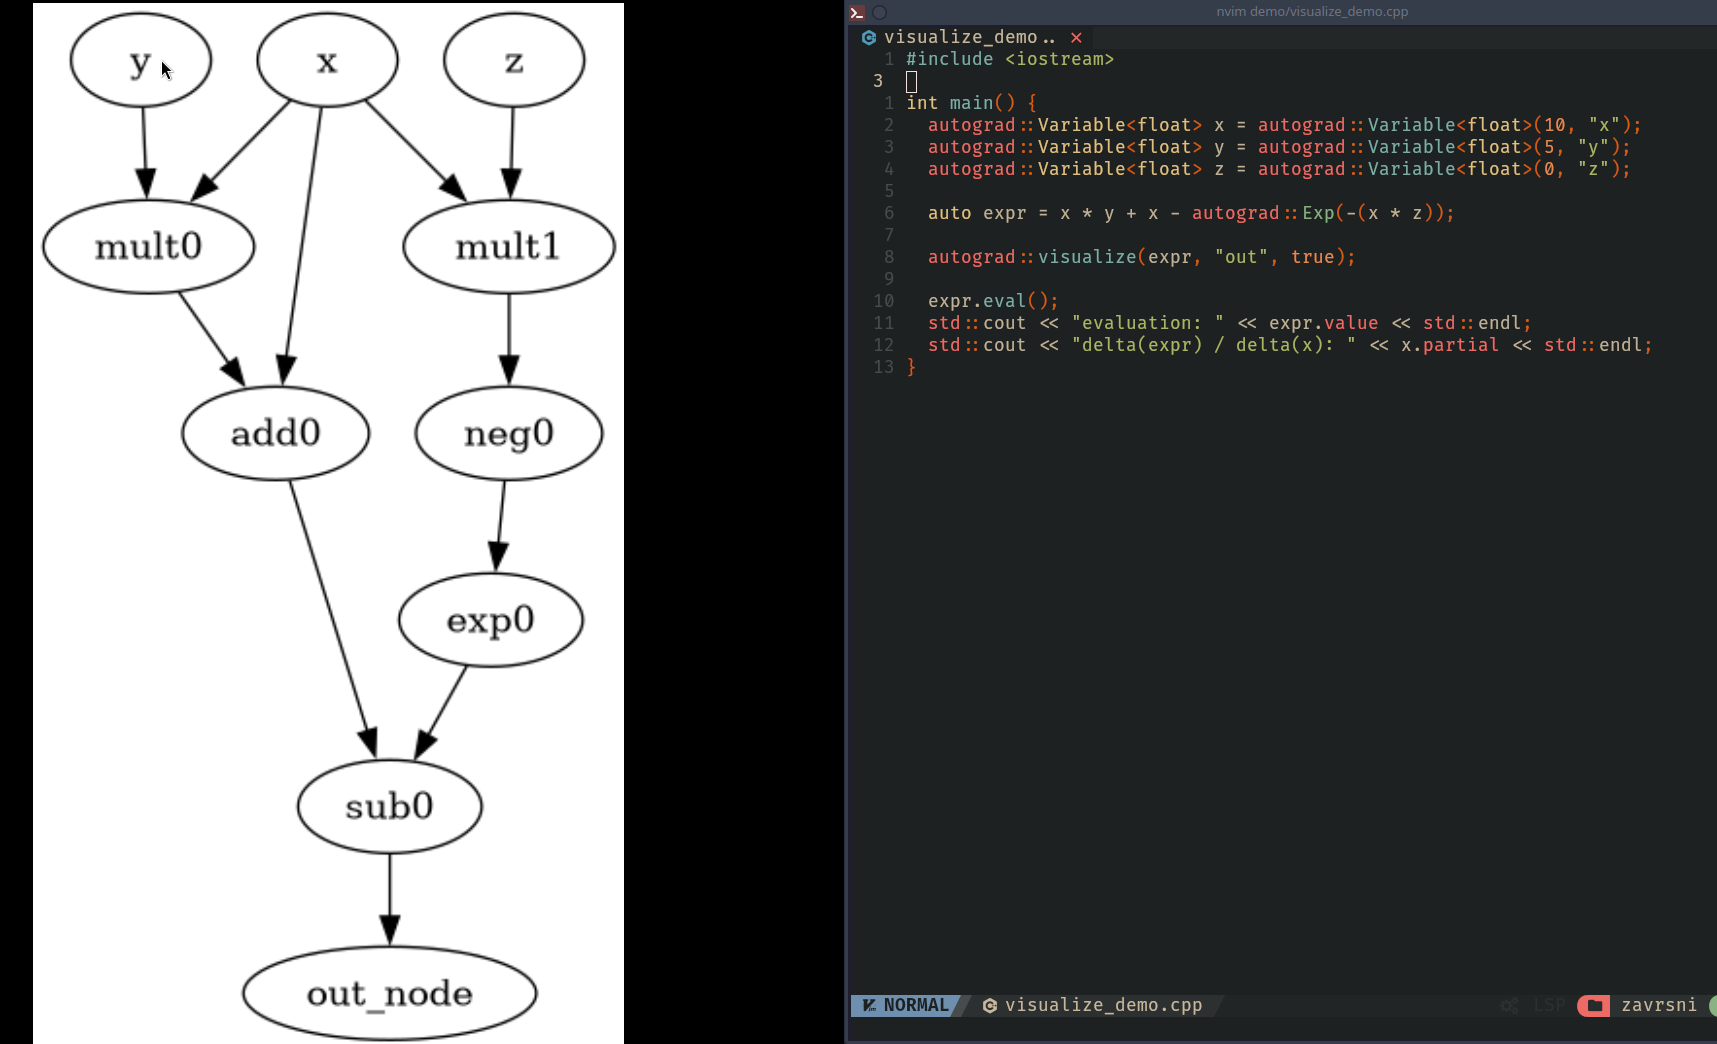
\includegraphics[width=0.7\linewidth]{../../pics/demo1.png}
  \caption{Primjer grafa funkcije: $f(x, y, z) = x * y + x - \exp(-x*z)$}
  \label{slk:graf_funkcije1}
\end{figure}
\\
Općenito, za neku funkciju: $f\colon \mathbb{R}^n \rightarrow \mathbb{R}^m$ vrijedi da će njezin graf imati $n$ čvorova varijabli, odnosno $n$ izvora te $m$ izlaznih čvorova, tj. $m$ ponora. Dodatno možemo pojednostaviti njezin graf ako funkciju zamislimo kao $f\colon \mathbb{V}^n \rightarrow \mathbb{V}^m$ te zatim predstavimo sve varijable kao vektore. Ta ideja će nam uvelike pojednostaviti samu implementaciju autograd programa jer će apstrahirati prijelaz s univarijatnih na multivarijatne funkcije.
\\
Sa slike \ref{slk:graf_funkcije1} možemo već naslutiti koja je glavna ideja algoritma; Glavna ideja jest da obiđemo zadani graf te u svakom čvoru odredimo derivaciju po pravilu ulančavanja:
\begin{equation}
  \frac{\partial (f_1 \circ (f_2 \circ \dotsb (f_{n-1} \circ f_n)))}{\partial x}
    = \frac{\partial f_1}{\partial f_2} \frac{\partial f_2}{\partial f_3}
      \dotsb
      \frac{\partial f_{n-1}}{\partial f_n} \frac{\partial f_n}{\partial x}
\end{equation}
\\
Čvorove u grafu možemo na slijedeći način predstaviti u objektnoj paradigmi (programski jezik \textit{Python}) \cite{wiki:autodiff}:
\lstset{language=python}
\begin{lstlisting}
class ValueAndPartial:
    def __init__(self, value, partial):
        self.value = value
        self.partial = partial

    def toList(self):
        return [self.value, self.partial]

class Expression:
    def __add__(self, other):
        return Plus(self, other)

    def __mul__(self, other):
        return Multiply(self, other)
\end{lstlisting}
\subsection{Forward mode}
Ovdje postoje dva pristupa: prvi, takozvani \textit{forward mode accumulation}, jest da počnemo od čvorova ulaza prema čvorovima izlaza, po formuli:
\begin{equation}
  \frac{\partial (f_{i-1} \circ f_i)}{\partial x} = \frac{\partial f_{i-1}}{\partial x} \frac{\partial f_i}{\partial f_{i-1}}
\end{equation}
\begin{figure}[h]
  \centering
  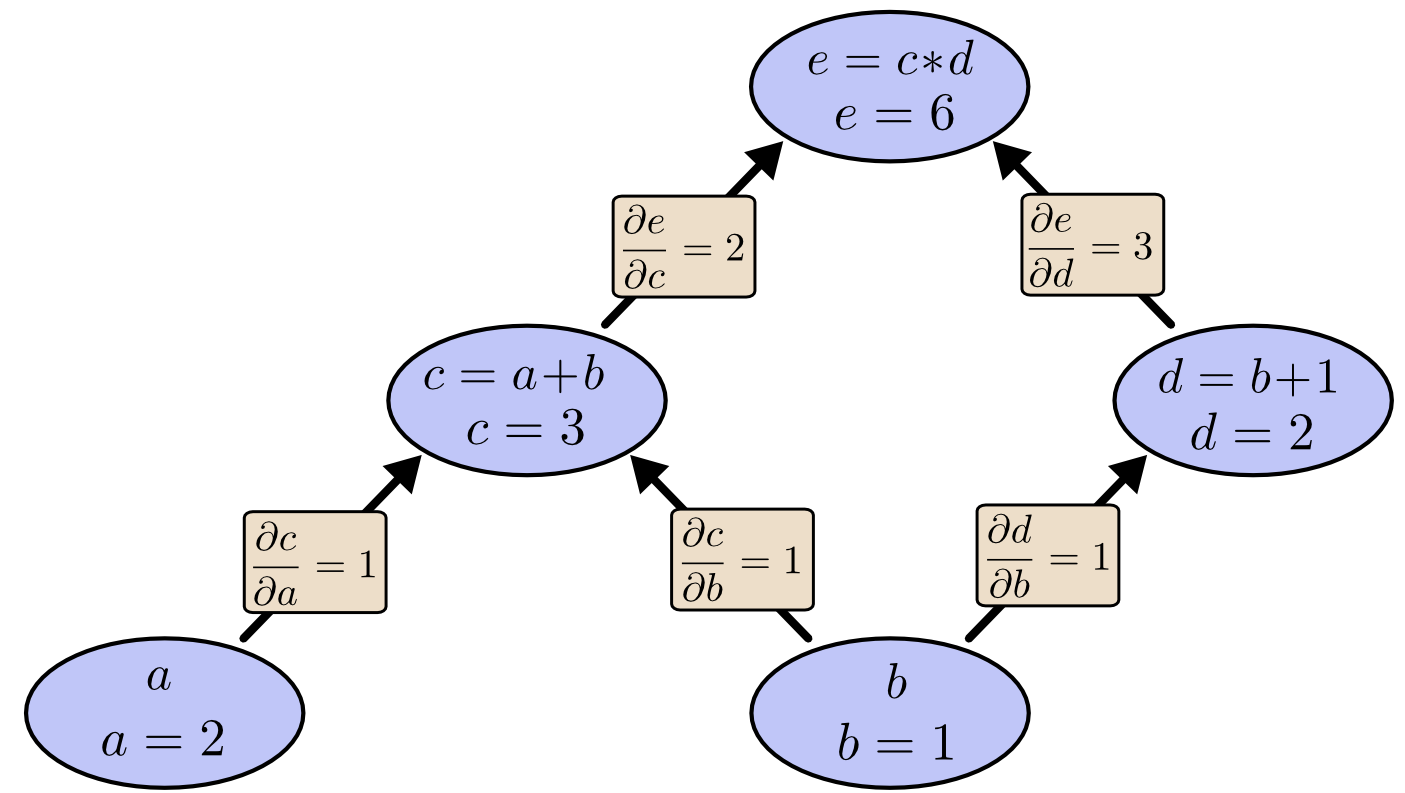
\includegraphics[width=0.7\linewidth]{"./slike/forward_graph.png"}
  \caption{Unaprijedni, \textit{forward mode accumulation} pristup}
  \cite{wuciawe_github}
  \label{slk:forward_graph}
\end{figure}
Vrijednost $f_{i-1}$ je u početku jednaka 1, a kasnije se propagira kroz slojeve grafa \ref{slk:forward_graph} kao vrijednost koju u literaturi često nazivaju \textit{seed value} (citation needed). Ovaj pristup je pogodan ukoliko je broj ulaza daleko manji od broja izlaza, odnosno vrijedi $f\colon \mathbb{R}^n \rightarrow \mathbb{R}^m. n << m$. Složenost ovog koda ovisi o strukturi grafa, no vidljivo je da prolazak kroz graf ponavljamo $n$ puta te je stoga poželjno da je $n$ mnogo manji od $m$. Ovaj pristup nije idealan za strojno učenje pošto je često ulazna domena mnogo veća od izlazne u toj primjeni.
\\
\begin{lstlisting}[caption={Primjer implementacije unaprijedne metode u programskom jeziku \textit{Python} \cite{wiki:autodiff}}]
class Variable(Expression):
    def __init__(self, value):
        self.value = value

    def evaluateAndDerive(self, variable):
        partial = 1 if self == variable else 0
        return ValueAndPartial(self.value, partial)

class Plus(Expression):
    def __init__(self, expressionA, expressionB):
        self.expressionA = expressionA
        self.expressionB = expressionB

    def evaluateAndDerive(self, variable):
        valueA, partialA = self.expressionA.evaluateAndDerive(variable).toList()
        valueB, partialB = self.expressionB.evaluateAndDerive(variable).toList()
        return ValueAndPartial(valueA + valueB, partialA + partialB)

class Multiply(Expression):
    def __init__(self, expressionA, expressionB):
        self.expressionA = expressionA
        self.expressionB = expressionB

    def evaluateAndDerive(self, variable):
        valueA, partialA = self.expressionA.evaluateAndDerive(variable).toList()
        valueB, partialB = self.expressionB.evaluateAndDerive(variable).toList()
        return ValueAndPartial(valueA * valueB, valueB * partialA + valueA * partialB)
\end{lstlisting}
\subsection{Reverse mode}
Drugi pristup problemu automatskog diferenciranja jest takozvani \textit{reverse mode accumulation}, tj. prolazak grafa unazad:
\begin{equation}
  \frac{\partial (f_i \circ f_{i+1})}{\partial x} = \frac{\partial f_{i+1}}{\partial f_i} \frac{\partial f_i}{\partial x}
\end{equation}
\begin{figure}[h]
  \centering
  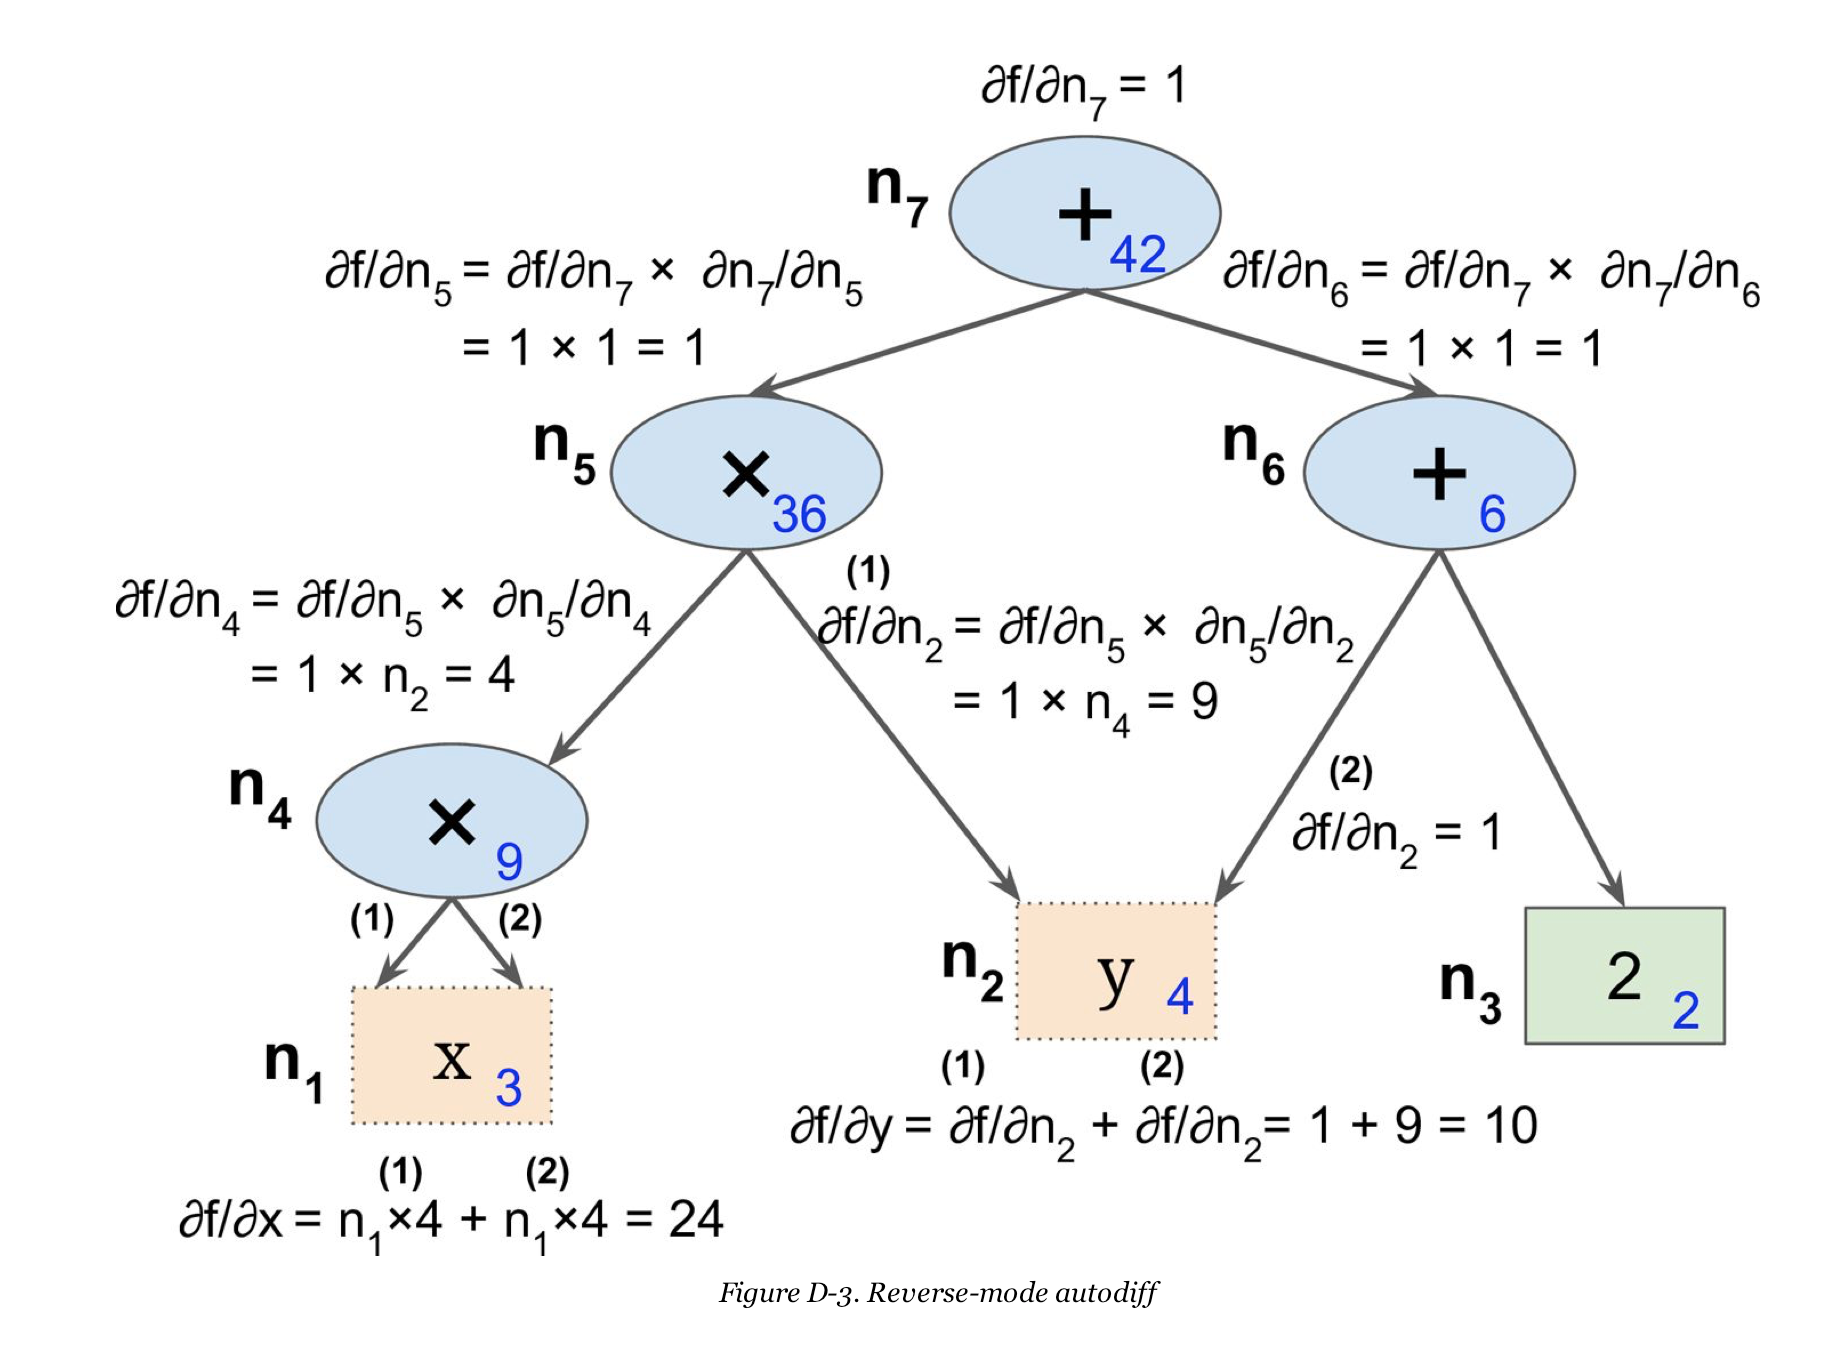
\includegraphics[width=0.7\linewidth]{"./slike/reverse_graph.png"}
  \caption{Unazadni, \textit{reverse mode accumulation} pristup}
  \cite{srijithr_gitlab}
  \label{slk:reverse_graf}
\end{figure}
U ovom pristupu se \textit{seed}-vrijednost šalje unazad kroz graf jednadžbe od ponora prema izvorima \ref{slk:reverse_graf}. Iz toga slijedi da će za neku funkciju $f\colon \mathbb{R}^n \rightarrow \mathbb{R}^m. m << n$ algoritam biti najefikasniji zato što će se $m$ puta pozvati funkcija prolaska kroz graf. Poseban slučaj ovog pristupa problemu automatskog diferenciranja jest temeljni princip koji se koristi za unazadnu propagaciju (\textit{eng. backpropagation}) u strojnom učenju (\textbf{citation needed}).
\\
Zanimljivo je da su oba algoritma optimalna samo za jednu određenu domenu primjene. To je zato što je problem izračuna Jakobijana za proizvoljnu funkciju $f\colon \mathbb{R}^n \rightarrow \mathbb{R}^m$ s minimalnim brojem računskih operacija problem koji je NP-potpun. Problem je poznat i kao \textit{optimal Jacobian problem} \cite{naumann:optimaljacobian}.
\begin{lstlisting}[caption={Primjer implementacije unazadne metode u programskom jeziku \textit{Python} \cite{wiki:autodiff}}]
class Variable(Expression):
    def __init__(self, value):
        self.value = value
        self.partial = 0

    def evaluate(self):
        pass

    def derive(self, seed):
        self.partial += seed

class Plus(Expression):
    def __init__(self, expressionA, expressionB):
        self.expressionA = expressionA
        self.expressionB = expressionB
        self.value = None

    def evaluate(self):
        self.expressionA.evaluate()
        self.expressionB.evaluate()
        self.value = self.expressionA.value + self.expressionB.value

    def derive(self, seed):
        self.expressionA.derive(seed)
        self.expressionB.derive(seed)

class Multiply(Expression):
    def __init__(self, expressionA, expressionB):
        self.expressionA = expressionA
        self.expressionB = expressionB
        self.value = None

    def evaluate(self):
        self.expressionA.evaluate()
        self.expressionB.evaluate()
        self.value = self.expressionA.value * self.expressionB.value

    def derive(self, seed):
        self.expressionA.derive(self.expressionB.value * seed)
        self.expressionB.derive(self.expressionA.value * seed)
\end{lstlisting}

\pagebreak
\section{Dualni brojevi}
Dualni brojevi su još jedan potenncijalni pristup za lako rješavanje prve derivacije jednadžbe. Iako nećemo koristiti ovaj pristup u implementaciji unazadnog (\textit{backward mode}) diferenciranja, valjalo bi ga spomenuti kao jednog od najintuitivnijih pristupa za rješavanje \textit{autodiffa} kod unaprijednog (\textit{forward mode}) diferenciranja. O čemu se radi?
\\
Zamislimo da bilo koji realni broj možemo zapisati kao dualni broj $x$ \cite{hoffmann2016hitchhiker}:
\begin{equation}
  \begin{split}
  x = a + b \varepsilon \\
  \varepsilon ^ 2 = 0, \varepsilon \ne 0 \\
  a, b \in \mathbb{R} \\
  \end{split}
  \label{eq:dualni}
\end{equation}
U formuli \ref{eq:dualni} broj $a$ predstavlja realni broj, početnu vrijednost neke varijable ili izraza, dok $b$ predstavlja diferencijal kojeg propagiramo od varijabli do rezultata određene funkcije. Ovakav pristup je memorijski jednostavniji jer ne zahtjeva slaganje složenih grafova, već računamo s sve kao i s "normalnim" brojevima. To vrijedi zato što se svaka analitička funkcija lako može proširiti u domenu dualnih brojeva preko svojeg Taylorovog reda \cite{hoffmann2016hitchhiker}:
\begin{equation}
  f(a + b \varepsilon) = \sum_{n=0}^{\infty} \frac{f^{(n)}(a) b^n \varepsilon^n}{n!} = f(a) + b f'(a) \varepsilon
\end{equation}
Jednostavna implementacija ove ideje za funkcije zbrajanja i množenja izleda ovako u programskom jeziku \textit{Python}:

\lstset{language=python}
\begin{lstlisting}[caption={Primjer korištenja dualnih brojeva za unaprijednu metodu \textit{autodiffa} \cite{wiki:autodiff}}]
class Dual:
    def __init__(self, realPart, infinitesimalPart=0):
        self.realPart = realPart
        self.infinitesimalPart = infinitesimalPart

    def __add__(self, other):
        return Dual(
            self.realPart + other.realPart,
            self.infinitesimalPart + other.infinitesimalPart
        )

    def __mul__(self, other):
        return Dual(
            self.realPart * other.realPart,
            other.realPart * self.infinitesimalPart + self.realPart * other.infinitesimalPart
        )

# Primjer: Gradijent funkcije: z = x * (x + y) + y * y at (x, y) = (2, 3)
def f(x, y):
    return x * (x + y) + y * y
x = Dual(2)
y = Dual(3)
epsilon = Dual(0, 1)
a = f(x + epsilon, y)
b = f(x, y + epsilon)
print("parcijalno z po x =", a.infinitesimalPart)  # Output: 7
print("parcijalno z po y =", b.infinitesimalPart)  # Output: 8
\end{lstlisting}

\pagebreak
\section{Pristupi implementaciji grafa}
\subsection{Nadjačavanje operatora}

Jedan način implementacije automatskog diferenciranja jest nadjačavanje operatora. To je način kojeg ćemo koristiti u ovom radu te koji je već bio pokazan u primjerima. Glavna ideja jest da imamo sučelje preko kojeg modeliramo izraz koji omogućava klijentu da zove metode \textit{derive()} i \textit{evaluate()}. Sve ostale operacije se realiziraju uz pomoć rekurzije, bilo unaprijedne ili unazadne, te nasljeđivanjem i implementacijom pravila ulančavanja za pojedine funkcije.
Klijent takav sustav može na jednostavan način koristiti ako smo nadjačali operatore za osnovne računske operacije (eng.\ \textit{operator overloading}). Ukoliko je to slučaj, klijent jednostavno može konstruirati varijable te zatim proizvoljne izrazi pisati bez da je svjestan pozadinskih operacija. Na takav način funkcionira Pytorchev \textit{torch.autograd}, koji je glavni modul zaslužan za automatsko diferenciranje \cite{docs:autograd}. Na slici \ref{slk:klasni} je prikazan klasni dijagram takve implementacije.
\\

\begin{figure}[h]
  \centering
  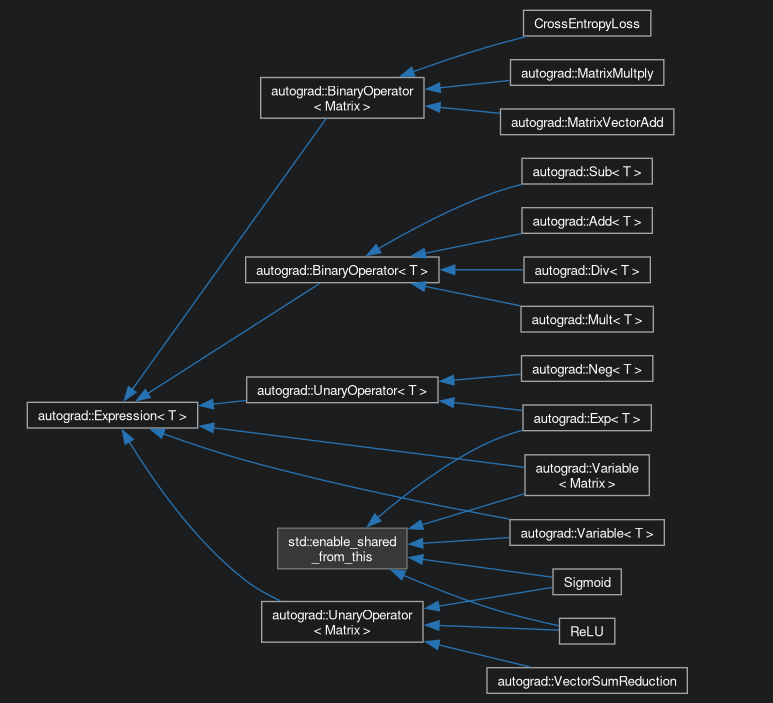
\includegraphics[width=0.7\linewidth]{./slike/klasni_dijagram.png}
  \caption{Klasni dijagram implementacije automatskog diferenciranja uz nadjačavanje operatora u objektnoj paradigmi}
  \label{slk:klasni}
\end{figure}

\subsection{Transformacija izvornog koda}

Drugi, efikasniji način jest umetanje međukoda, kojeg optimirajući prevoditelj može dodatno obraditi kasnije, u naš kod, odnosno klijentov kod. Glavna ideja jest da imamo okvir koji matematičke izraze izravno prevodi u međukod za evaluaciju (zamjena za metodu \textit{evaluate()}) te međukod za derivaciju (zamjena za metodu \textit{derive()}). Ukoliko imamo takav okvir, klijent može lako preko njega prevesti matematičke izraze te njihov izračun umetnuti u svoj kod. To se opet može ostvariti preko objektnog modela. Primjer razvojnog okvira koji koristi ovakav pristup jest TensorFlow i Zygote.jl \cite{prague:diffcpp}. Zygote.jl koristi llvm međukod kako bi izravno, na temelju neke ulazne funkcije, izgenerirao naredbe u strojno neovisnom kodu niske razine koji se kasnije lako može optimirati:
\\

\begin{lstlisting}[caption={Primjer korištenja Zygote.jl za generiranje llvm međukoda za funkciju: $a^2 + a*b$ \cite{prague:diffcpp}}]
function P1(a::Float64, b::Float64) :: Float64 
    return a^2 + a*b 
end

@code_llvm P1(0.1, 1.0) 
; a*a 
%2 = fmul double %0, %0 
; a*b 
%3 = fmul double %0, %1 
; a*a + a*b 
%4 = fadd double %2, %3 
ret double %4 
 
@code_llvm gradient(P1, 0.1, 1.0) 
; gradient = [2*a + b, a] 
; a + a 
 %3 = fadd double %1, %1 
; 2*a + b 
 %4 = fadd double %3, %2 
 %.sroa.0.0..sroa_idx = getelementptr inbounds [2 x double], [2 x double]* 
%0, i64 0, i64 0 
; Res[0] = 2*a + b 
store double %4, double* %.sroa.0.0..sroa_idx, align 8 
 %.sroa.2.0..sroa_idx4 = getelementptr inbounds [2 x double], [2 x double]* 
%0, i64 0, i64 1 
; Res[1] = a  
store double %1, double* %.sroa.2.0..sroa_idx4, align 8 
ret void
\end{lstlisting}

\pagebreak
\section{OpenCL i C++}
\textbf{TODO:} napiši nekaj tu...
\\
\blindtext


%-------------------------------------------------------------------------------
\chapter{Glavni dio}
\label{pog:glavni_dio}

\section{Autograd\_core implementacija}
\textbf{TODO:} opiši jezgrenu funkcionalnost i zakaj je taksa
\blindtext

\pagebreak
\section{Matrix calculus}
\textbf{TODO:} opiši matrične operacije i poveži ih s matematičkom analizom
\blindtext

\pagebreak
\section{OpenCL + autograd\_core}
\textbf{TODO:} opiši kak si povezal opencl i autograd core implementaciju
\blindtext

\pagebreak
\section{Demonstracijski programi}
\textbf{TODO:} izdvoji najbitnije demonstracijske programe koje si napisal
\blindtext

%-------------------------------------------------------------------------------
\chapter{Rezultati i rasprava}
\label{pog:rezultati_i_rasprava}

\section{Usporedba s pytorchem}
\textbf{TODO:} usporedi brzinu izvođenja demonstracijskih programa s pytorch ekvivalentima
\blindtext

\pagebreak
\section{Moguće optimizacije}
\textbf{TODO:} piši o mogućim optimizacijama pretraživanja grafa. recimo odsjecanje grana itd.
\blindtext

\pagebreak
\section{Budući rad}
\textbf{TODO:} opiši kaj si mogel još dodati u smislu featurea
\cite{123DCatch}
\blindtext


%--- ZAKLJUČAK / CONCLUSION ----------------------------------------------------
\chapter{Zaključak}
\label{pog:zakljucak}

Zaključno, TODO...
\blindtext


%--- LITERATURA / REFERENCES ---------------------------------------------------

% Literatura se automatski generira iz zadane .bib datoteke / References are automatically generated from the supplied .bib file
% Upiši ime BibTeX datoteke bez .bib nastavka / Enter the name of the BibTeX file without .bib extension
\bibliography{literatura}



%--- SAŽETAK / ABSTRACT --------------------------------------------------------

% Sažetak na hrvatskom
\begin{sazetak}
  \textbf{TODO:} Unesite sažetak na hrvatskom.
  \blindtext
\end{sazetak}

\begin{kljucnerijeci}
  \textbf{TODO:} ključčne riječi
  prva ključna riječ; druga ključna riječ; treća ključna riječ
\end{kljucnerijeci}


% Abstract in English
\begin{abstract}
  This is the abstract in english. \textbf{TODO:} write a proper one...
  \blindtext
\end{abstract}

\begin{keywords}
  the first keyword; the second keyword; the third keyword
\end{keywords}


%--- PRIVITCI / APPENDIX -------------------------------------------------------

% Sva poglavlja koja slijede će biti označena slovom i riječi privitak / All following chapters will be denoted with an appendix and a letter
\backmatter

\end{document}
